\documentclass[12pt]{article}
\usepackage[a4paper, total={6in, 8.5in}]{geometry}
\usepackage{graphicx}
\graphicspath{ {images/output/} }
\usepackage{amsmath}
\usepackage{minted}
\usepackage{multicol}
\usepackage{caption}
\usepackage[english]{babel}
\usepackage{placeins}
\usepackage{titling}


\begin{document}
\vspace*{\fill}
\begin{center}

    \emph{Heaven's Light is Our Guide} \\
    \textbf{Rajshahi University of Engineering and Technology} \\

    \begin{figure}[H]
        \centering
        
\includegraphics[scale=.34]{images/RUET_logo.png}
        \label{fig:ruet_logo}
    \end{figure}
    \vspace{5mm}

    \textbf{Course Code}\\
    ECE 3112\\
    \vspace{3mm}
    \textbf{Course Title}\\
    Microprocessor, Assembly Language \& Interfacing Sessional

    \vspace{5mm}
    \textbf{Experiment Date:} {April 22, 2024},\\
    \textbf{Submission Date:} {April 29, 2024}\\

    \vspace{5mm}
    \textbf{Lab Report 1, 2 \& 3: Using Assembly Language to Program 8086 Microprocessor to do Different Tasks.}

    \vspace{15mm}

    \begin{tabular}{c|c}
        \textbf{Submitted to} & \textbf{Submitted by} \\
        Md. Omaer Faruq Goni  & Md. Tajim An Noor     \\
        Lecturer              & Roll: 2010025         \\
        Dept of ECE, Ruet     &                       \\
    \end{tabular}

\end{center}
\vspace*{\fill}

\clearpage
\title{Conversion From Lowercase to Uppercase.}
\author{}
\date{}
\maketitle

\section*{Tools Used}
\begin{itemize}
    \item emu8086 - 8086 Microprocessor Emulator
    \item MacTeX -\LaTeX  compiler.
    \item VS Code with \LaTeX workshop extension as a text editor.
\end{itemize}

\section*{Process}

\subsection*{Code:}
\begin{minted}[breaklines, linenos]{gas}
DATA    SEGMENT
    CR EQU 0DH
    LF EQU 0AH
    MSG1 DB 'ENTER A LOWERCASE LETTER: $'
    MSG2 DB CR,LF, 'IN UPPER CASE IT IS: '
    CHAR DB ?, '$'
DATA    ENDS
CODE    SEGMENT
    ASSUME CS:CODE, DS:DATA
    
START:  
    MOV AX, DATA
    MOV DS, AX
          
    LEA DX, MSG1
    MOV AH, 9
    INT 21h
    MOV AH, 1
    INT 21h
    
    SUB AL, 20H
    MOV CHAR, AL
        
    LEA DX,MSG2
    MOV AH, 9
    INT 21h

    MOV AH, 4CH
    INT 21h    
     
CODE    ENDS

END START
\end{minted}

\subsection*{Output}
\begin{center}
    \centering
    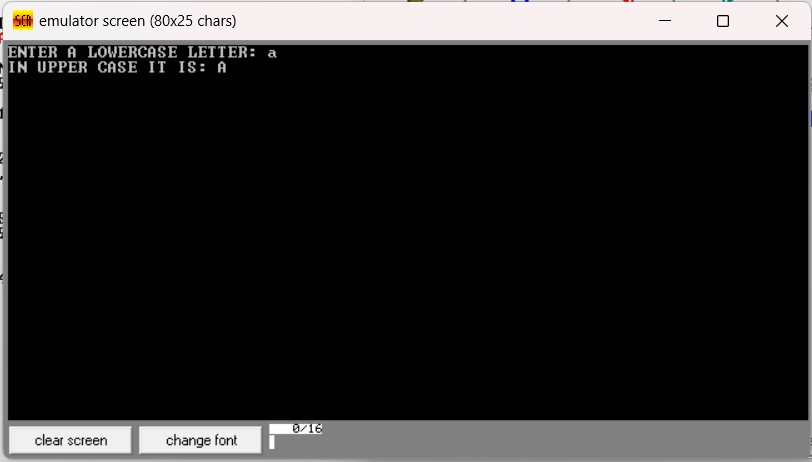
\includegraphics[width = .8\textwidth]{MALI1.jpg}
    \captionof{figure}{Lowercase to Uppercase}
\end{center}


\clearpage
\title{Conversion From Uppercase to Lowercase.}
\author{}
\date{}
\maketitle

\section*{Tools Used}
\begin{itemize}
    \item emu8086 - 8086 Microprocessor Emulator
    \item MacTeX -\LaTeX  compiler.
    \item VS Code with \LaTeX workshop extension as a text editor.
\end{itemize}

\section*{Process}

\subsection*{Code:}
\begin{minted}[breaklines, linenos]{gas}
    DATA    SEGMENT
    CR EQU 0DH
    LF EQU 0AH
    MSG1 DB 'ENTER A UPPERCASE LETTER: $'
    MSG2 DB CR,LF, 'IN LOWERCASE IT IS: '
    CHAR DB ?, '$'
DATA    ENDS
CODE    SEGMENT
    ASSUME CS:CODE, DS:DATA
    
START:  
    MOV AX, DATA
    MOV DS, AX
          
    LEA DX, MSG1
    MOV AH, 9
    INT 21h
    MOV AH, 1
    INT 21h
    
    ADD AL, 20H
    MOV CHAR, AL
        
    LEA DX,MSG2
    MOV AH, 9
    INT 21h

    MOV AH, 4CH
    INT 21h    
     
CODE    ENDS

END START
\end{minted}

\subsection*{Output}
\begin{center}
    \centering
    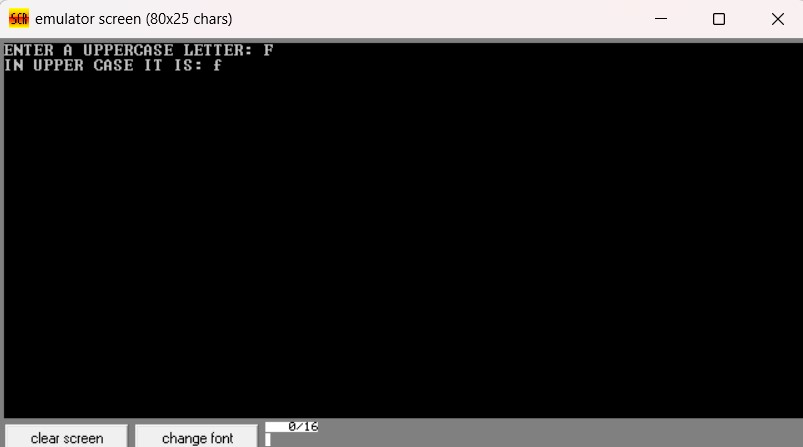
\includegraphics[width = .8\textwidth]{MALI2.jpg}
    \captionof{figure}{Uppercase to Lowercase}
\end{center}



\clearpage
\title{Adding Two Numbers}
\author{}
\date{}
\maketitle

\section*{Tools Used}
\begin{itemize}
    \item emu8086 - 8086 Microprocessor Emulator
    \item MacTeX -\LaTeX  compiler.
    \item VS Code with \LaTeX workshop extension as a text editor.
\end{itemize}

\section*{Process}

\subsection*{Code:}
\begin{minted}[breaklines, linenos]{gas}
DATA    SEGMENT
    CR EQU 0DH
    LF EQU 0AH

    MSG1 DB 'ENTER FIRST NUMBER: $'
    NUM1 DB ?
    MSG2 DB CR,LF,'ENTER SECOND NUMBER: $'
    NUM2 DB ?
    MSG3 DB CR, LF, 'SUM = '
    NUM3 DW ?,'$'
DATA    ENDS

CODE    SEGMENT
    ASSUME CS:CODE, DS:DATA
    
START: 
    MOV AX, DATA
    MOV DS, AX
           
    LEA DX, MSG1
    MOV AH, 9
    INT 21h
    
    MOV AH, 1
    INT 21h
    SUB AL, '0'  
    MOV NUM1, AL
    
    LEA DX, MSG2
    MOV AH, 9
    INT 21h
    
    MOV AH, 1
    INT 21h
    SUB AL, '0' 
    MOV NUM2, AL
    
    MOV BH,0
    MOV BL, NUM1
    MOV AH, 0  
    MOV AL, NUM2
    ADD AX,BX
    MOV NUM3, AX
    
    ADD NUM3, '0'
    
    LEA DX, MSG3
    MOV AH, 9
    INT 21h
    
    MOV AH, 4CH
    INT 21h
     
CODE    ENDS

END START
\end{minted}

\subsection*{Output}
\begin{center}
    \centering
    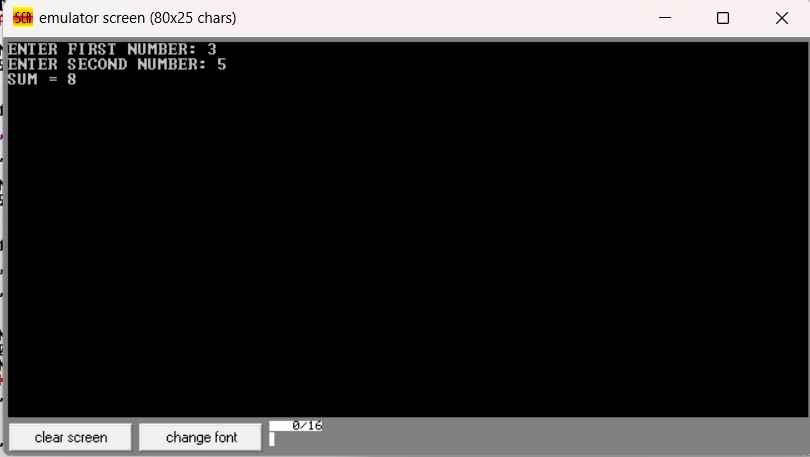
\includegraphics[width = .8\textwidth]{MALI3.jpg}
    \captionof{figure}{Uppercase to Lowercase}
\end{center}


\section*{Keywords}
\begin{description}
    \item[CR, LF] Carriage Return \& Line Feed. Both together is used to go to the next line. CR is used to go to next line and LF to go to the start of the line.
    \item[DB] Data Byte. Used to declare type of variable.
    \item[MOV] Move. Used to move data from the second register to the first.
    \item[LEA] Load Effective Address. Used to finding address of variable, and addition or subtraction without affecting flags.
    \item[INT 21h] Interrupt. Used to give emu8086 take back control.
    \item[SUB] Subtract. Used to subtract the second value from the first one and store in the first one.
    \item[]
\end{description}

\bibliographystyle{IEEEtran}
\bibliography{ref}

\end{document}
